\section{Predicción del Nivel del Río Paraguay mediante LSTM}
\vspace{0.3cm}
\justify
Antes de construir los modelos de predicción de precios, se necesitaba contar con una proyección confiable del nivel del río Paraguay, variable que opera como entrada exógena en los modelos posteriores. Para esto se entrenó un modelo LSTM siguiendo tres etapas: búsqueda automática de hiperparámetros con Optuna, entrenamiento del modelo final con la configuración óptima y generación del pronóstico a 730 días consecutivos.

\subsection{Serie Histórica y Partición de los Datos}

\justify
La serie contiene registros diarios del nivel del río Paraguay en el Puerto de Asunción, abarcando el período de enero de 2014 a julio de 2025.

\justify
Las estadísticas descriptivas de la variable muestran una media de 2,63 m y una desviación estándar de 2,17 m, con valores entre $-1{,}61$ m y $7{,}88$ m. La Figura \ref{fig:serie_historica} muestra la serie completa, donde se aprecia la alternancia entre períodos de crecida y estiaje con amplitudes marcadamente distintas entre años.

\begin{figure}[H]
    \centering
    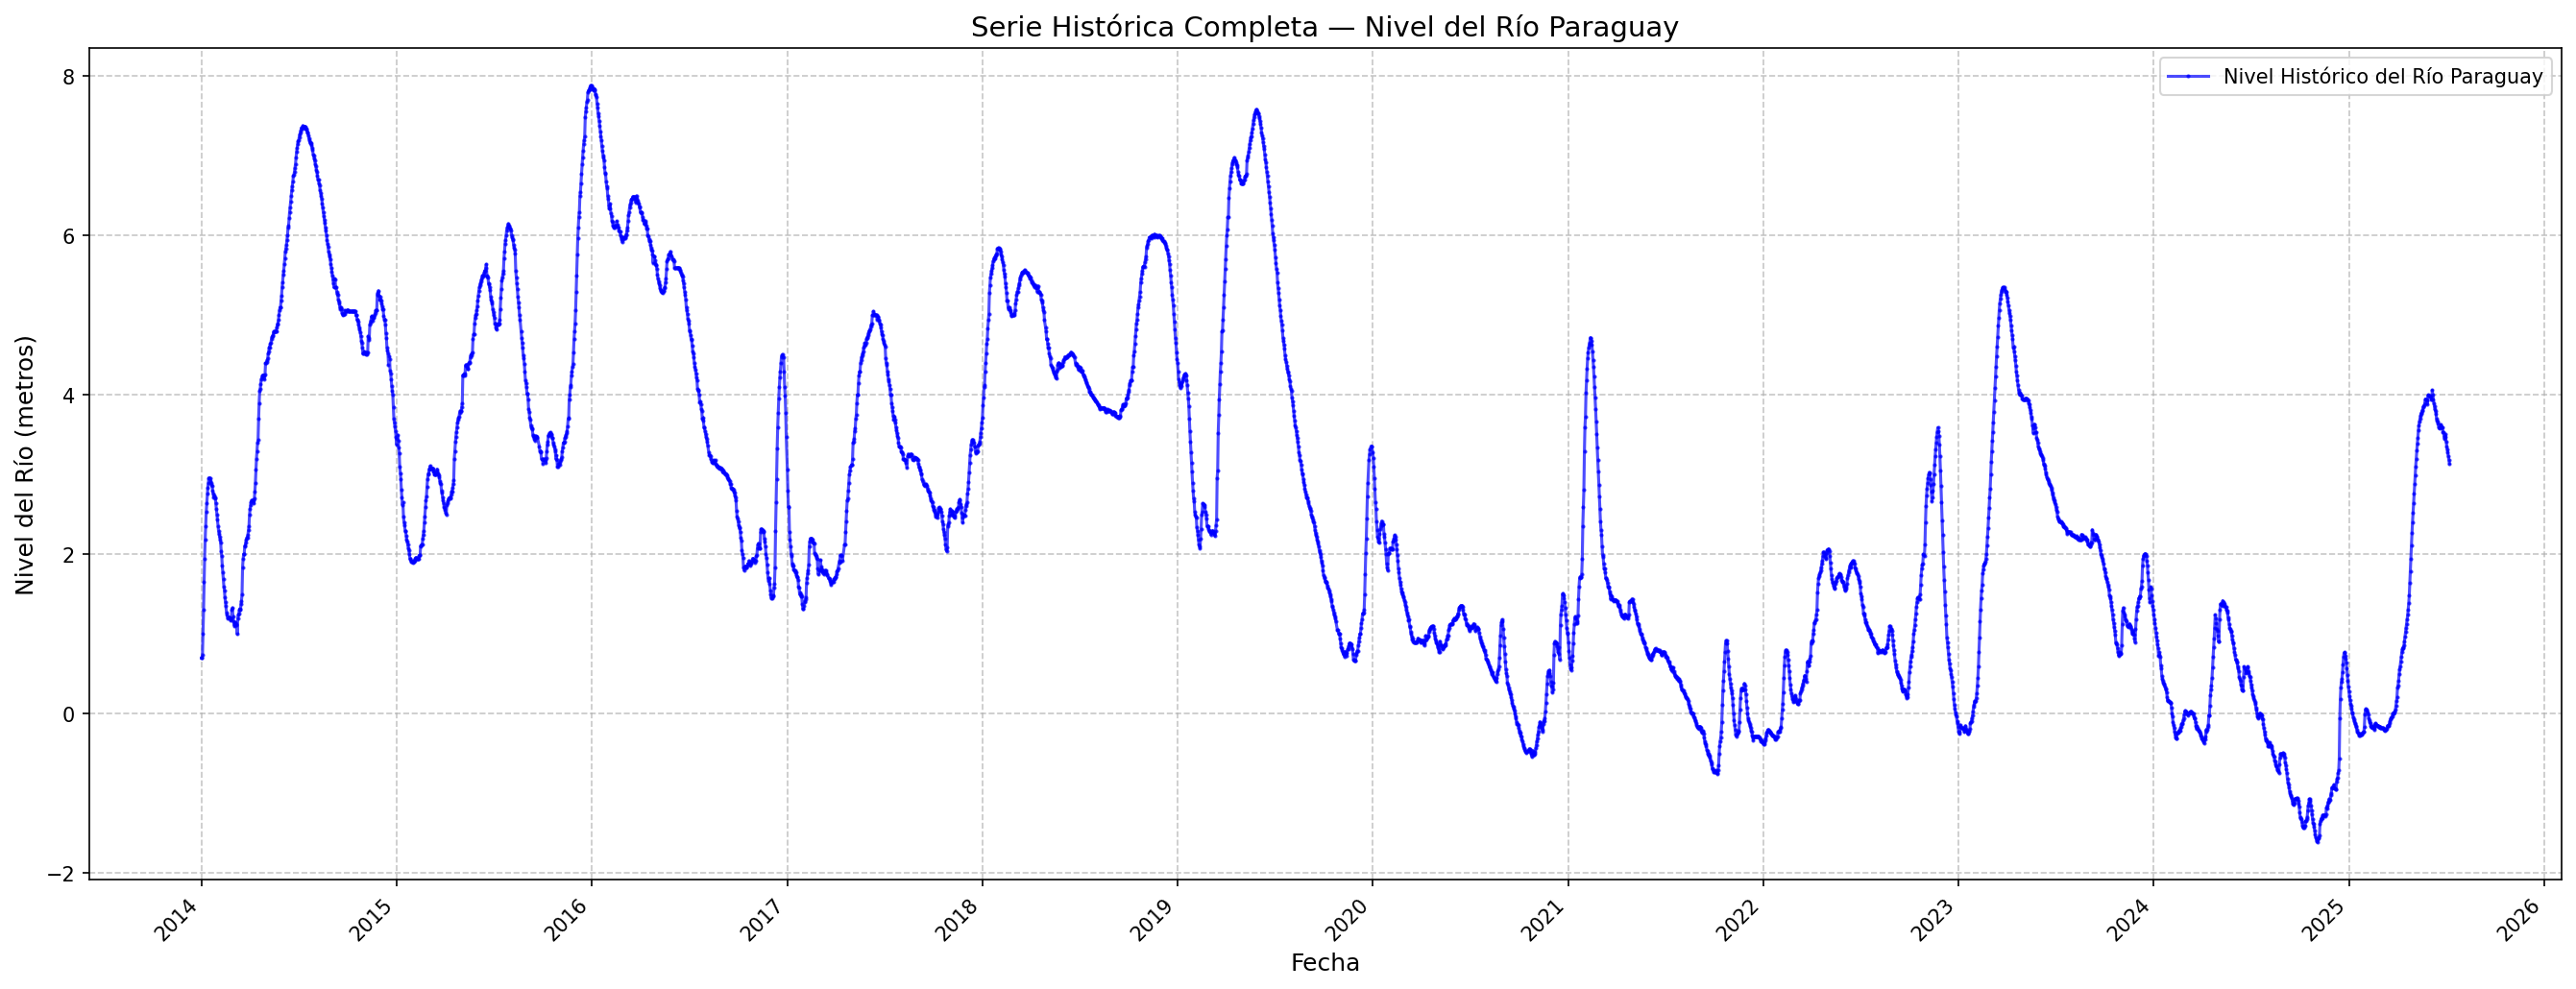
\includegraphics[width=\textwidth]{predicciones/prediccion_nivel_rio/resultados/grafico_00_serie_historica.png}
    \caption{Serie histórica completa del nivel diario del río Paraguay (2014--2025).}
    \label{fig:serie_historica}
\end{figure}

\justify
El modelo recibe 12 variables de entrada por paso de tiempo: el nivel del río más siete características temporales y cuatro de anomalía. Las temporales incluyen representaciones cíclicas del día del año, el mes y la estación (codificadas como seno y coseno), más el año normalizado. Las de anomalía capturan desviaciones respecto a medias móviles de 30 y 90 días, y tendencias de 7 y 30 días.

\justify
La partición del dataset siguió un criterio estrictamente cronológico. El conjunto de entrenamiento comprende desde el 1 de enero de 2014 hasta el 22 de enero de 2022 (2.944 observaciones, aproximadamente el 70\% del total); el de validación, desde el 23 de enero de 2022 hasta el 14 de octubre de 2023 (630 observaciones, el 15\%); y el de prueba, desde el 15 de octubre de 2023 hasta el 7 de julio de 2025 (632 observaciones, el 15\% restante). Al aplicar la ventana de lookback de 30 días al conjunto de entrenamiento, el número efectivo de secuencias se reduce a 2.914. Esta proporción fue seleccionada por ser la que produjo el mejor resultado en experimentos previos con distintas configuraciones de partición. La Figura \ref{fig:particiones} muestra la distribución temporal de los tres subconjuntos.

\begin{figure}[H]
    \centering
    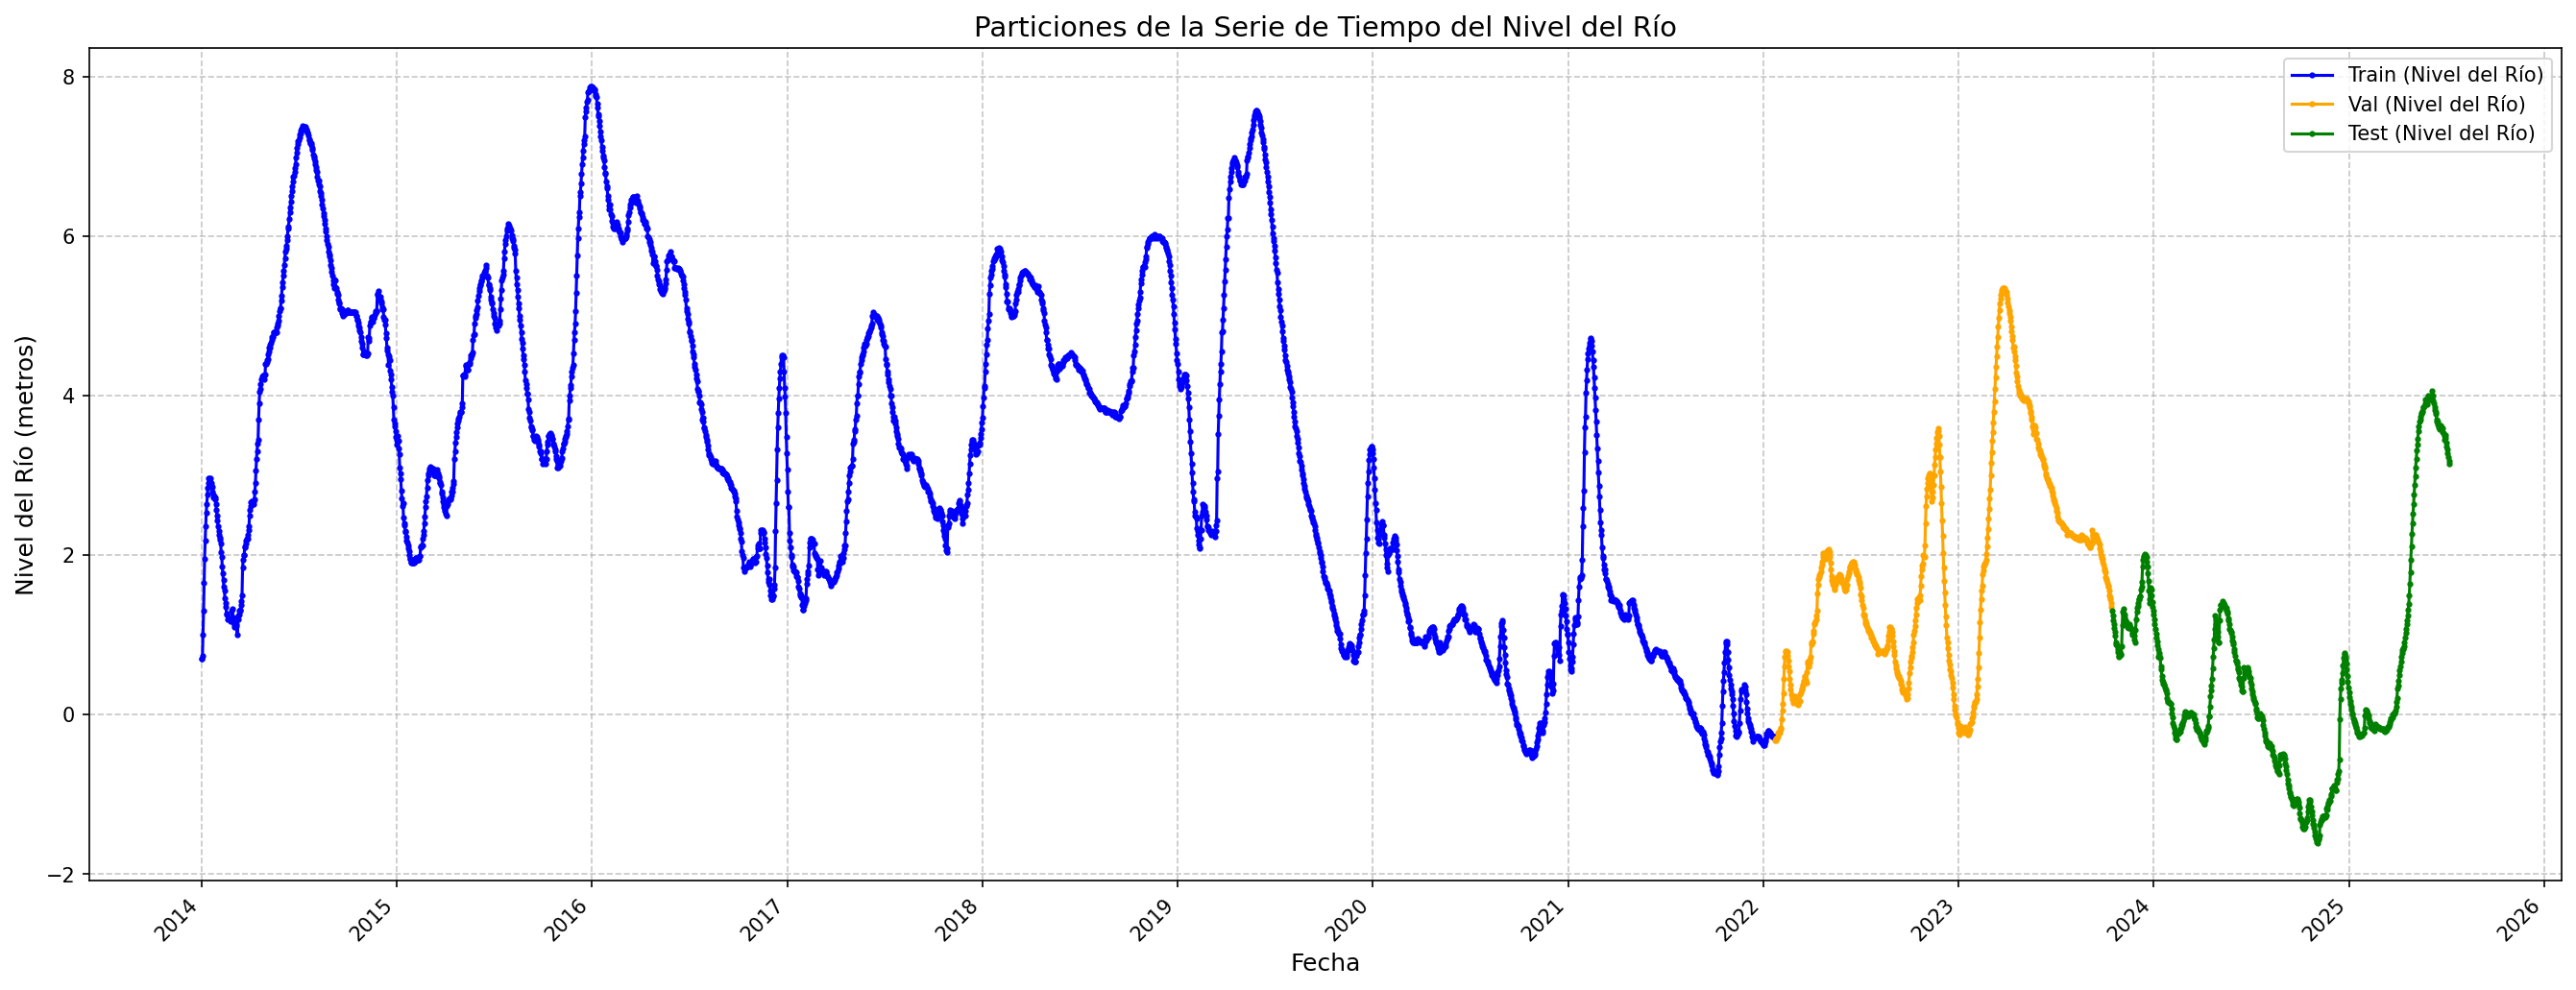
\includegraphics[width=\textwidth]{predicciones/prediccion_nivel_rio/resultados/grafico_01_particiones.png}
    \caption{Partición cronológica de la serie: entrenamiento (azul), validación (naranja) y prueba (verde).}
    \label{fig:particiones}
\end{figure}

\subsection{Optimización de Hiperparámetros con Optuna}

\justify
La búsqueda de hiperparámetros se realizó con Optuna, usando el sampler TPE (\textit{Tree-structured Parzen Estimator}) y poda de trials con \textit{MedianPruner} para descartar tempranamente las configuraciones claramente inferiores. Se evaluaron 300 trials, proceso que demandó 278 minutos en total. El mejor RMSE de validación obtenido fue de 0,0371 m.

\justify
Los hiperparámetros óptimos se resumen en la Tabla \ref{tab:hiperparametros_lstm_rio}.

\begin{table}[H]
    \centering
    \caption{Hiperparámetros óptimos del modelo LSTM para la predicción del nivel del río Paraguay.}
    \label{tab:hiperparametros_lstm_rio}
    \begin{tabular}{lc}
        \toprule
        \textbf{Hiperparámetro} & \textbf{Valor óptimo} \\
        \midrule
        Número de capas LSTM       & 1 \\
        Unidades ocultas           & 512 \\
        Bidireccional              & No \\
        Tasa de \textit{dropout}   & 0,05 \\
        Activación capa densa      & Lineal \\
        Ventana de lookback        & 30 días \\
        Estrategia de predicción   & Recursiva \\
        Optimizador                & Adam \\
        Tasa de aprendizaje        & 0,006079 \\
        \textit{Weight decay}      & $4{,}70 \times 10^{-7}$ \\
        Tamaño de lote (\textit{batch size}) & 256 \\
        Planificador de LR         & CosineAnnealingLR \\
        \bottomrule
    \end{tabular}
\end{table}

\justify
La configuración óptima corresponde a una sola capa LSTM con 512 unidades ocultas. La estrategia recursiva fue preferida sobre la directa, lo que indica que el modelo aprovecha mejor la retroalimentación acumulada paso a paso para proyecciones largas. El total de parámetros entrenables es de 1.075.713.

\subsection{Entrenamiento del Modelo Final}

\justify
El modelo final fue entrenado durante 99 épocas con los hiperparámetros óptimos, una ventana de lookback de 30 días y una paciencia de 30 épocas para la detención temprana. La Figura \ref{fig:curva_aprendizaje} presenta la evolución del error de entrenamiento y validación a lo largo del proceso.

\begin{figure}[H]
    \centering
    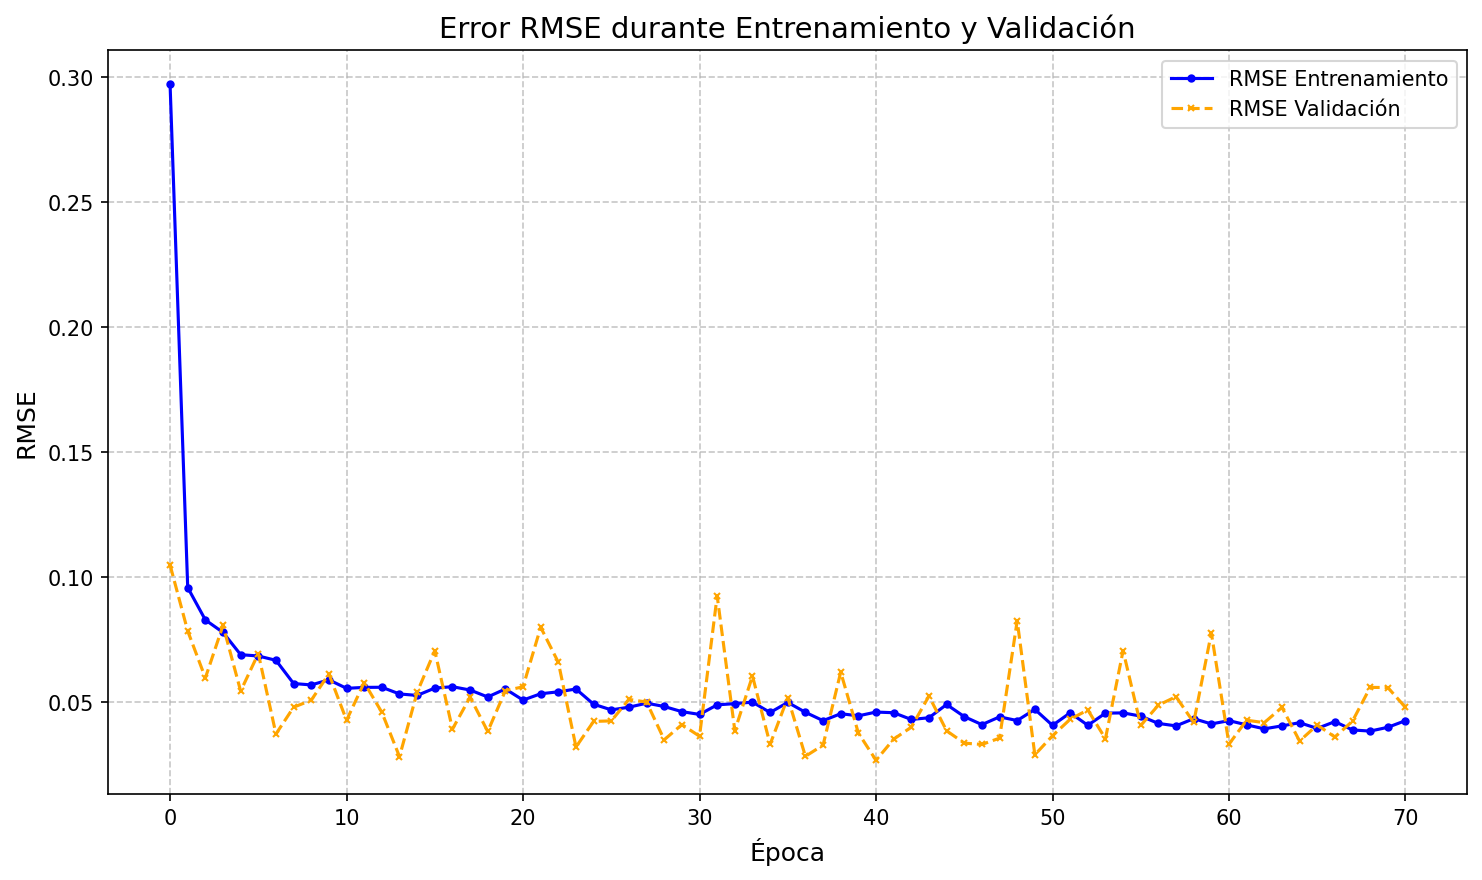
\includegraphics[width=0.85\textwidth]{predicciones/prediccion_nivel_rio/resultados/grafico_04_curva_aprendizaje.png}
    \caption{Curva de aprendizaje del modelo LSTM: RMSE de entrenamiento y validación por época.}
    \label{fig:curva_aprendizaje}
\end{figure}

\justify
Durante las primeras épocas, la pérdida cae rápidamente desde valores en torno a 0,30 hasta situarse por debajo de 0,10. A partir de la época 15 aproximadamente, el error de entrenamiento se estabiliza alrededor de 0,04 a 0,05, mientras el de validación oscila en rangos similares sin mostrar una tendencia ascendente sostenida, lo que indica que no se produjo sobreajuste significativo.

\subsection{Métricas de Evaluación}

\justify
La Tabla \ref{tab:metricas_lstm_rio} presenta el RMSE en los tres subconjuntos.

\begin{table}[H]
    \centering
    \caption{RMSE del modelo LSTM para el nivel del río Paraguay en los conjuntos de entrenamiento, validación y prueba.}
    \label{tab:metricas_lstm_rio}
    \begin{tabular}{lc}
        \toprule
        \textbf{Conjunto} & \textbf{RMSE (m)} \\
        \midrule
        Entrenamiento  & 0,0479 \\
        Validación     & 0,0373 \\
        Prueba         & 0,0457 \\
        \bottomrule
    \end{tabular}
\end{table}

\justify
El error en el conjunto de prueba es de 4,57 cm, sobre una variable que oscila entre $-1{,}61$ m y $7{,}88$ m. Este nivel de precisión, inferior a 5 cm sobre un rango de casi 10 metros, confirma la capacidad del modelo LSTM para reproducir la dinámica hidrológica del río Paraguay con alta fidelidad.

\subsection{Predicción del Nivel del Río a 730 Días}

\justify
Concluida la evaluación, se generó la predicción del nivel diario para un horizonte de 730 días mediante la estrategia recursiva: el modelo predice el valor del día siguiente ($t+1$) a partir de la ventana de 30 días previos, incorpora ese valor a la secuencia y repite el proceso hasta completar 730 pasos desde el último dato disponible (7 de julio de 2025, nivel = 3,14 m). Para reducir la acumulación de error en horizontes largos, la predicción se combina gradualmente con la climatología histórica a través de un factor de mezcla $\alpha(t)$ que decrece desde 1,00 en el primer paso hasta valores próximos a 0 hacia el final del horizonte ($\alpha = 0{,}72$ a los 30 días, $\alpha = 0{,}37$ a los 90 días, $\alpha = 0{,}14$ a los 180 días).

\justify
La Figura \ref{fig:historico_prediccion} muestra la serie histórica completa junto con la predicción generada y la climatología histórica como referencia estacional.

\begin{figure}[H]
    \centering
    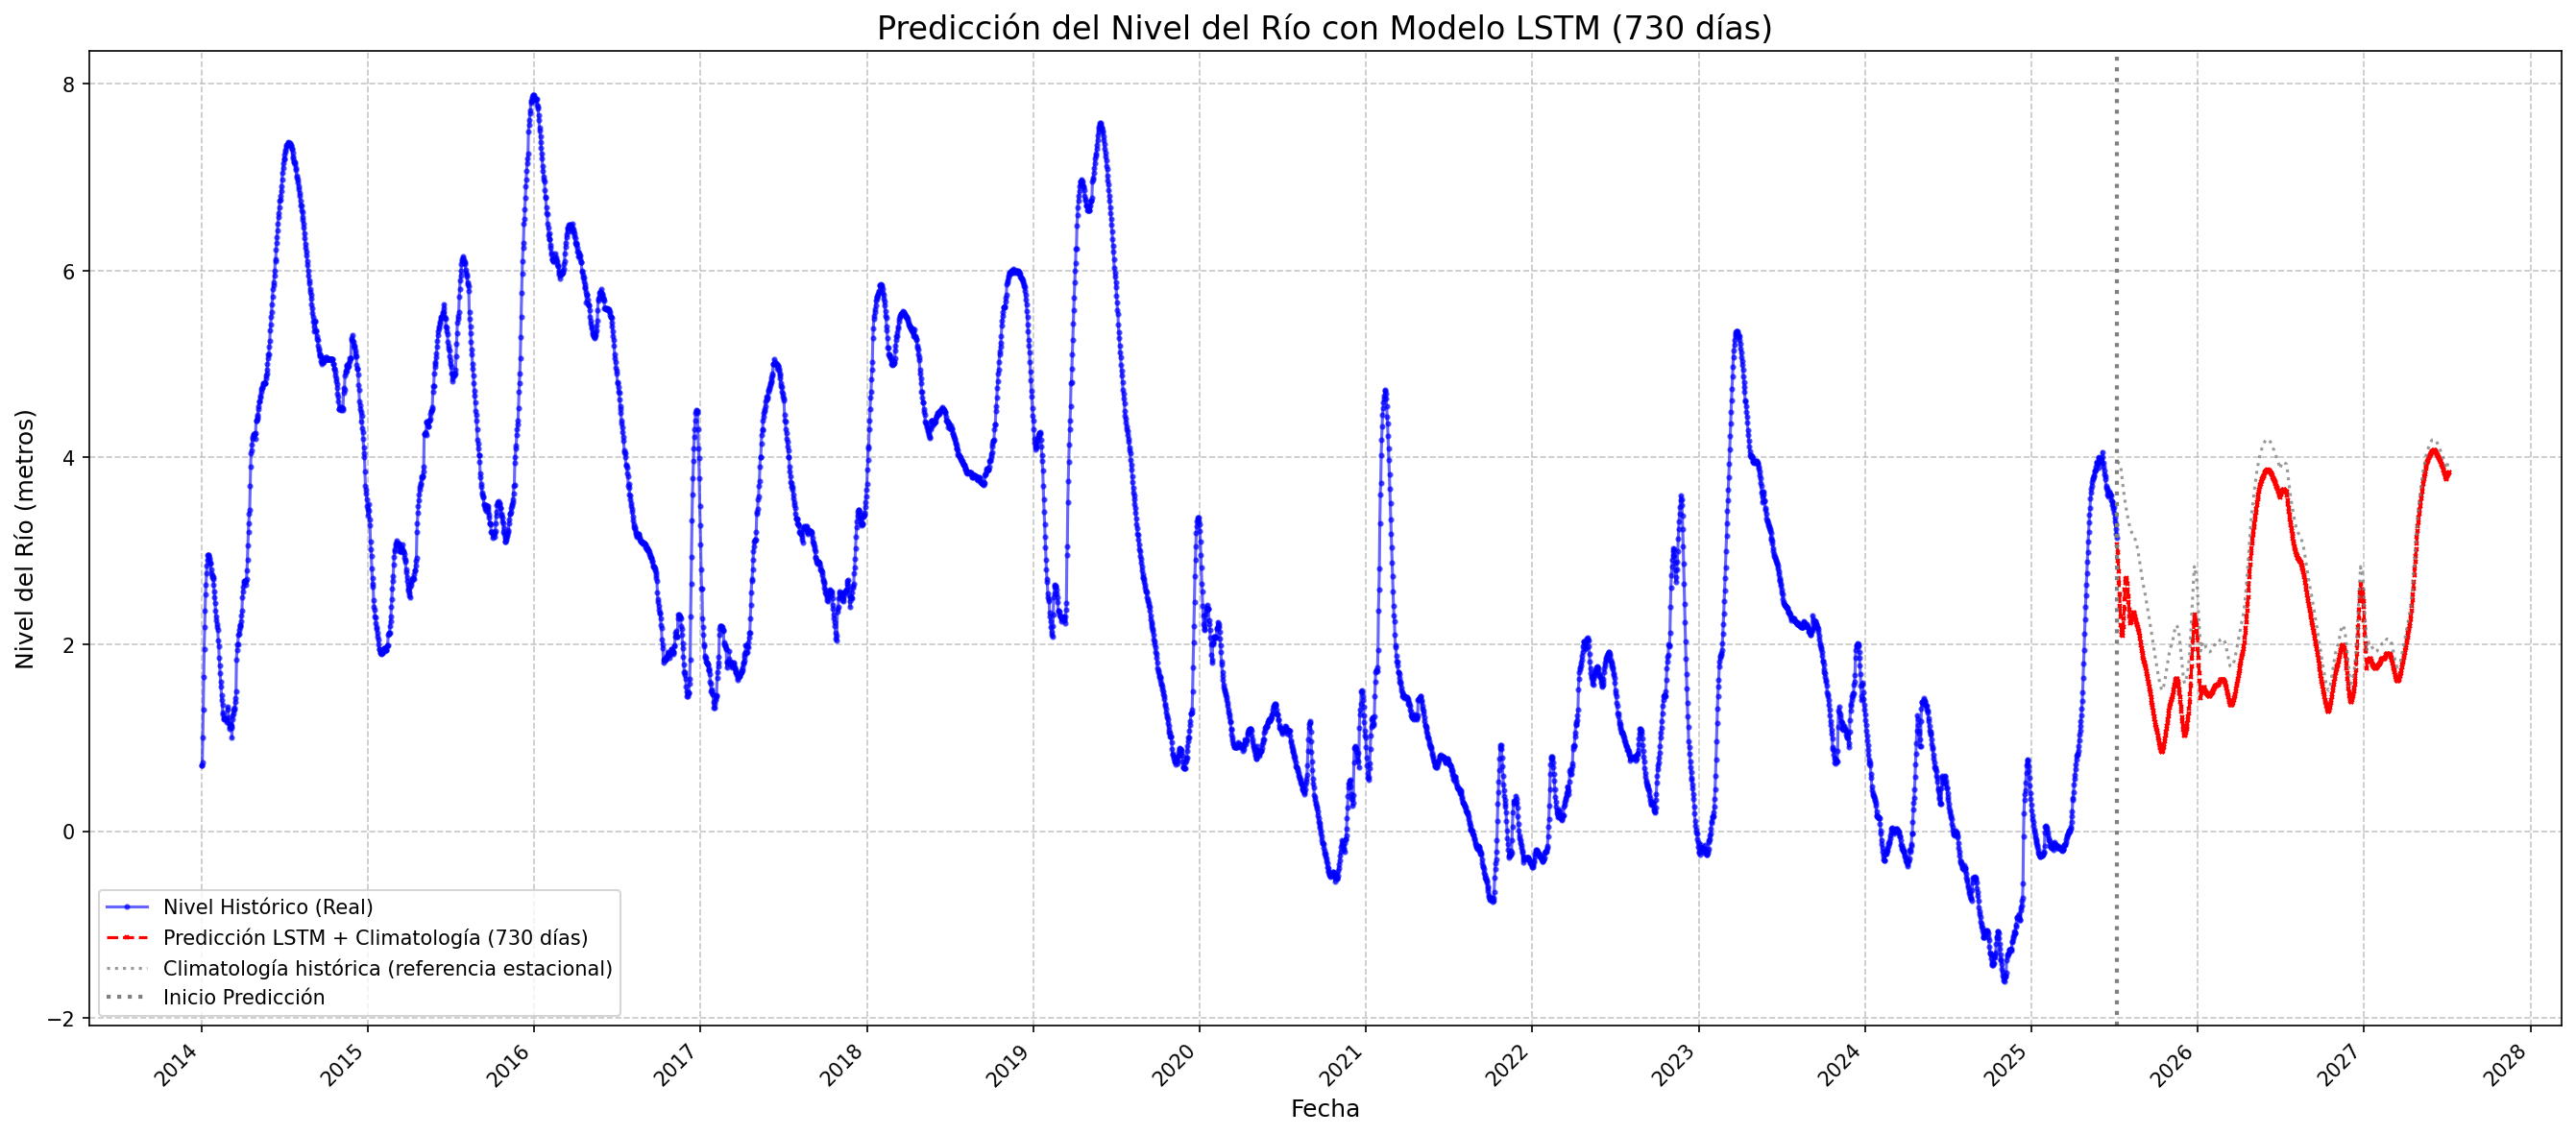
\includegraphics[width=\textwidth]{predicciones/prediccion_nivel_rio/resultados/grafico_08_historico_mas_prediccion.png}
    \caption{Serie histórica del nivel del río Paraguay y predicción LSTM a 730 días (julio 2025 -- julio 2027).}
    \label{fig:historico_prediccion}
\end{figure}

\justify
La Figura \ref{fig:zoom_transicion} muestra en detalle la transición entre datos reales (últimos 6 meses, en azul) y el inicio de la predicción (primeros 6 meses proyectados, en rojo). A partir del 8 de julio de 2025, el modelo proyecta un descenso progresivo desde los 3,08 m iniciales hasta un mínimo de aproximadamente 0,88 m hacia mediados de octubre de 2025, seguido de una recuperación que alcanza los 2,31 m hacia fines de diciembre de 2025, patrón consistente con el ciclo estacional del río.

\begin{figure}[H]
    \centering
    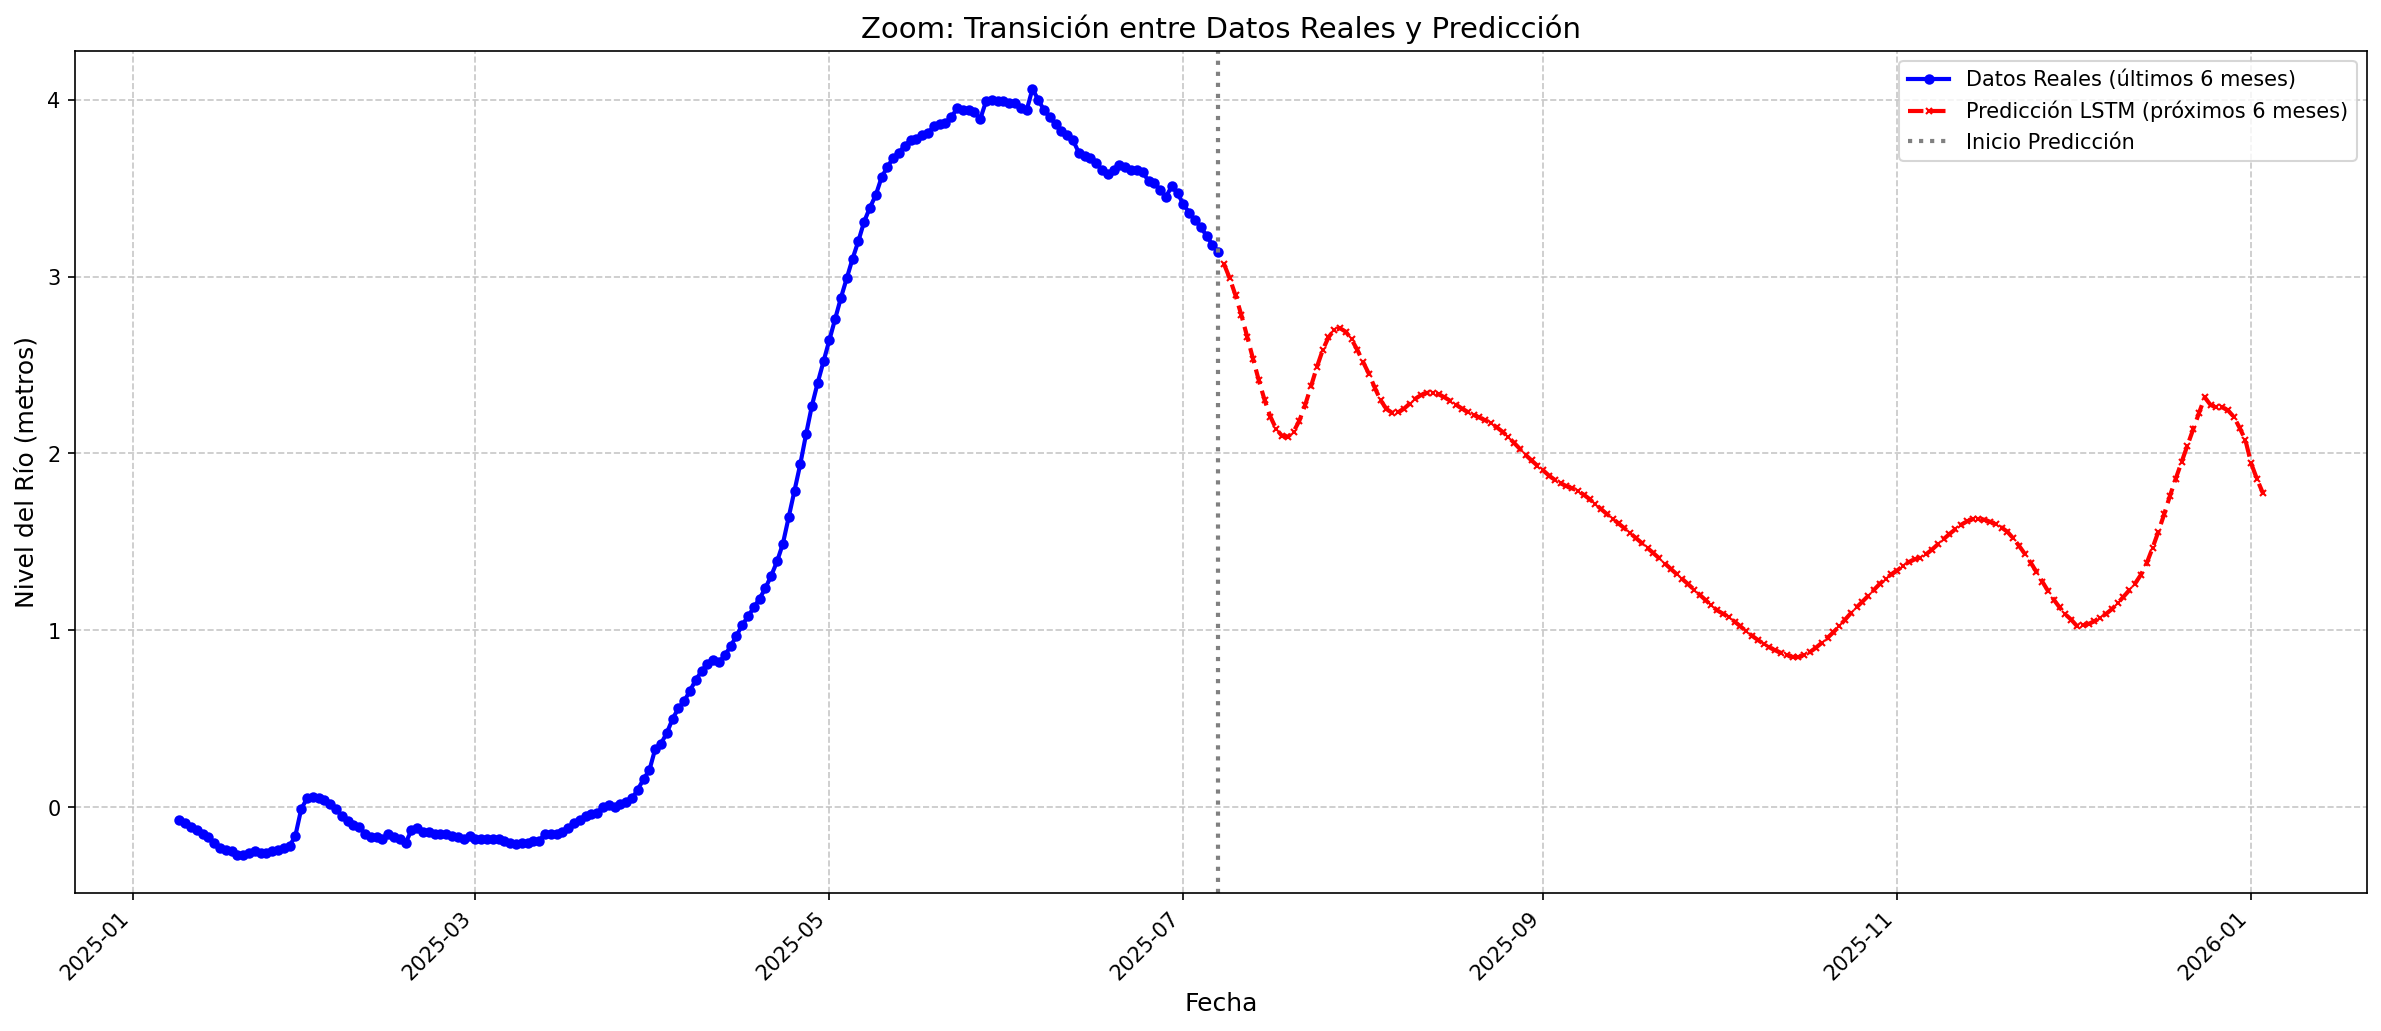
\includegraphics[width=\textwidth]{predicciones/prediccion_nivel_rio/resultados/grafico_09_zoom_transicion.png}
    \caption{Zoom en la transición entre datos reales y predicción LSTM: últimos 6 meses reales y primeros 6 meses proyectados.}
    \label{fig:zoom_transicion}
\end{figure}

\justify
La Figura \ref{fig:climatologia_prediccion} compara la predicción a 730 días con la climatología histórica tanto en la vista temporal de la proyección como en el ciclo estacional anual suavizado.

\begin{figure}[H]
    \centering
    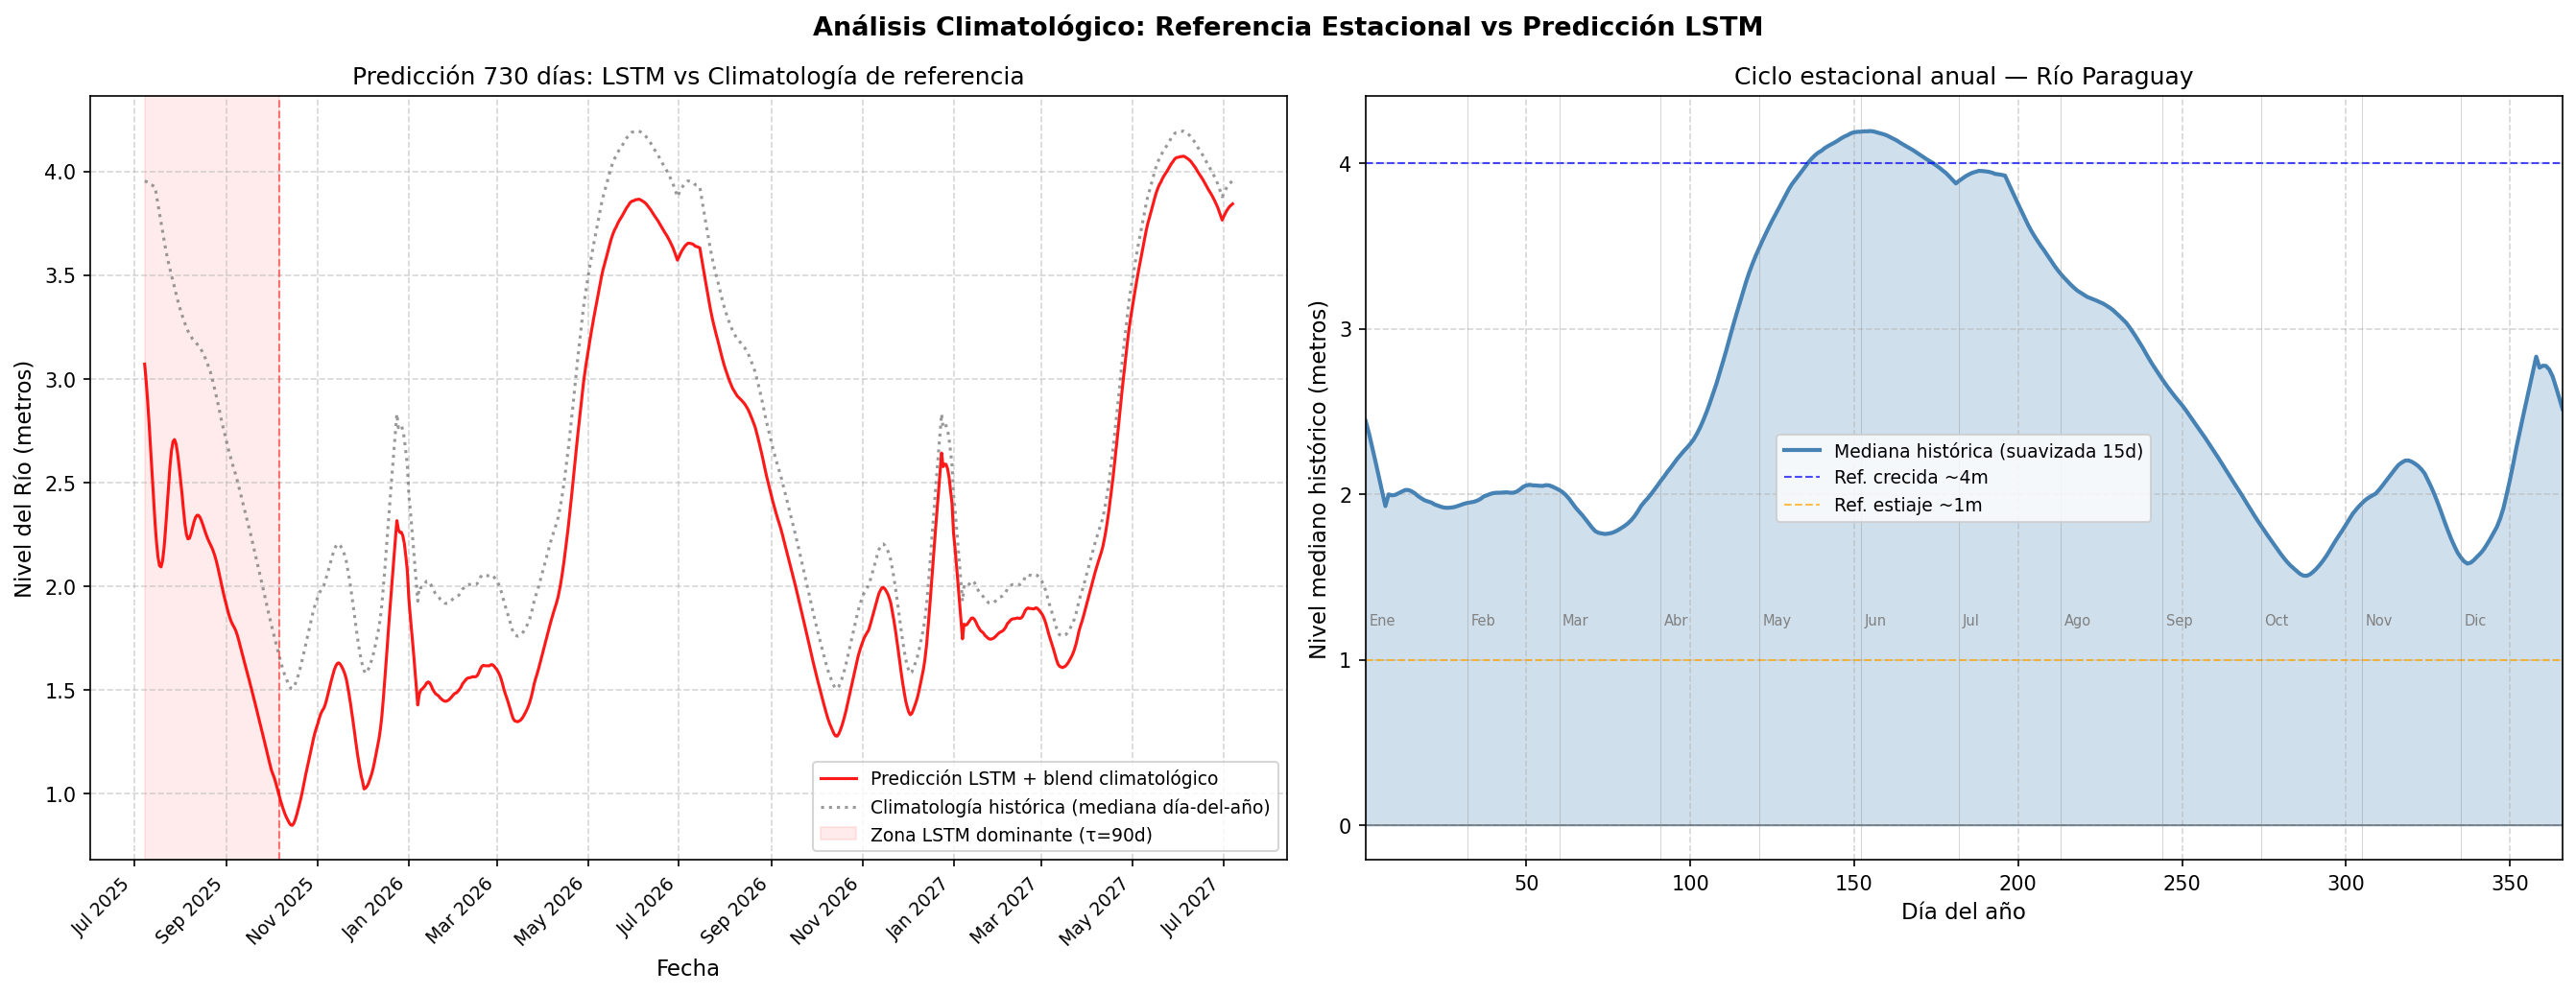
\includegraphics[width=\textwidth]{predicciones/prediccion_nivel_rio/resultados/grafico_11_climatologia_prediccion.png}
    \caption{Comparación entre la predicción LSTM a 730 días y la climatología histórica de referencia estacional.}
    \label{fig:climatologia_prediccion}
\end{figure}

\justify
La predicción a 730 días presenta un mínimo de 0,88 m, un máximo de 4,07 m, una media de 2,27 m y una desviación estándar de 0,90 m. El patrón estacional se reproduce en ambos años proyectados, con crecidas hacia los meses de mayo a julio y estiajes entre septiembre y noviembre. La amplitud de oscilación es algo menor que la de la climatología histórica, lo cual es esperable dado el blending progresivo con la climatología y la acumulación de incertidumbre en horizontes extendidos. Estos resultados validan la utilidad del modelo para estimar la variable exógena requerida por los modelos de predicción de precios de materiales de construcción.
